X-ray absorption (XAS) and Auger electron spectroscopies (AES) are powerful tools to study the electronic structure and the nearest environment of atoms and molecules in gas, liquid and solid phase. Understanding how atoms or molecules respond to irradiation with x-rays gives insight into the structure of solutions (Ref.\ \citep{smith17:13909} and references therein), and the mechanisms of radiation damage \citep{ONeill02:329,Carugo05:213,Stumpf16:237}. Upon absorption of an x-ray photon, either core excited or core ionized states of a specific atom are populated depending on the photon energy. The relaxation of these highly energetic states involves an ultrafast cascade of intraatomic processes, such as radiative and Auger decays, and it depends on the character of the initially populated states \citep{stoychev08:074307,Demekhin08:043421,Demekhin09:104303,Ouchi11:053415,Miteva14:164303,travnikova16:213001,Gokhberg14:661,Trinter14:664}. Furthermore, if the initially excited or ionized species is embedded in an environment, interatomic processes %such as charge and energy transfer 
are possible  \citep{Pokapanich09:7264,Pokapanich11:13430,Stumpf16:237,unger17:708,ceolin17:263003}.


In a solution, the course of such electronic decay cascades initiated by x-ray photoabsorption differs from that in atomic and molecular clusters due to the shorter distances and stronger interatomic interactions.
%In particular, the solvent molecules have two effects -- first, they affect the intensity and character of the excited \citep{miteva16:16671} or ionized states of the ion and second, they can participate in the decay processes, leading to the population of charge-separated final states, and ionization of the surrounding environment \citep{Pokapanich09:7264,Pokapanich11:13430,Stumpf16:237,ceolin17:263003,unger17:708}. Moreover, a process of internal ionization of the initially excited electron can also occur in aqueous solutions on a femtosecond to sub-femtosecond time scale \citep{Nordlund07:217406,Ottosson11:13489}. {\color{blue}Going to the tender and hard x-ray regimes, the lifetimes of the core ionized or core excited states become shorter compared to the case of water, on the order of 1\,fs. And thus, it is even more imperative to reveal whether the delocalization of the core excited electron occurs within the lifetime of the core hole.}
In this work we used AES together with XAS in the tender x-ray regime to study the electronic decay processes following x-ray absorption of aqueous potassium chloride at the K-edges of both \ki~and \cli. In particular, we demonstrate experimentally that at photon energies below the K-edges of the two ions, core excited states are populated. These states undergo resonant Auger decay within less than 1\,fs \citep{ceolin17:263003}. Although the \ki~and \cli~ions are isoelectronic, they have different fingerprints in the resonant Auger spectra. We demonstrate that these differences result from different electronic structures of the two ions, thus confirming that the combination of XAS and AES techniques is a sensitive probe of the electronic structure of solutions.


\begin{figure}
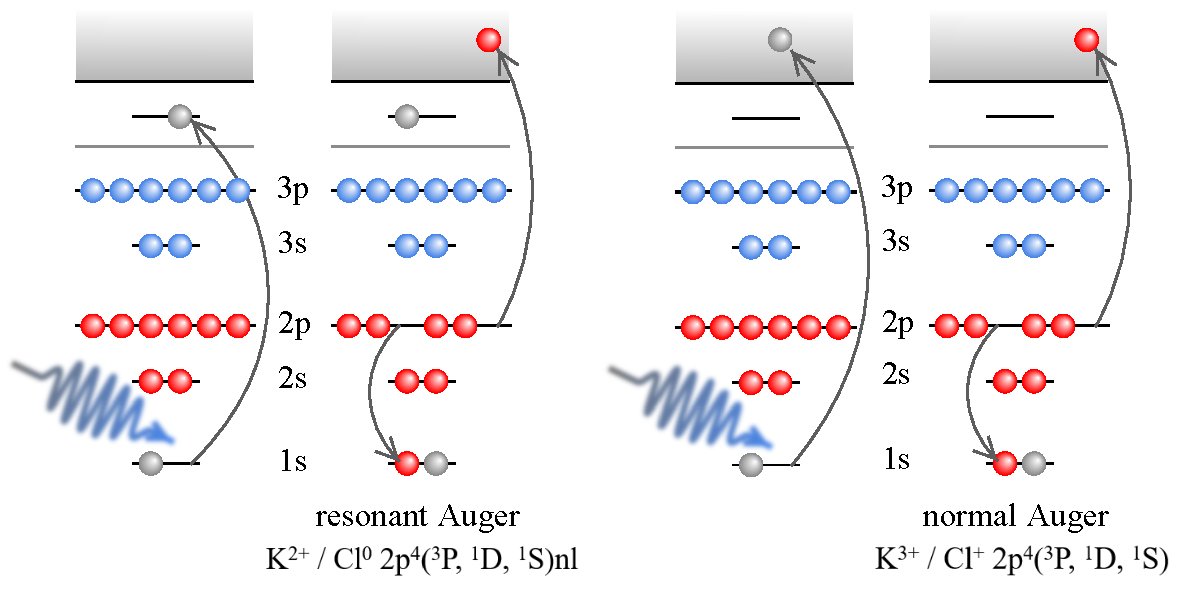
\includegraphics[scale=0.8]{figures/auger_process.pdf}
\caption{Schematic representation of the resonant (left) and normal (right) Auger processes of the isoelectronic \ki~and \cli~ions.}
\label{fg:auger}
\end{figure}

The resonant and normal Auger processes which we investigated in this work are schematically shown on Fig.\ \ref{fg:auger}. The KL$_{2,3}$L$_{2,3}$ normal Auger decay following K-shell ionization of aqueous \ki~and \cli~populates the 2p$^{-2}$($^3$P, $^1$D, $^1$S) final states. The $^3$P final states have a very low intensity since the corresponding transitions are forbidden from angular momentum and parity conservation rules. In the case of K$^{+}_{\text{aq}}$ the maxima of the $^1$S and $^1$D KL$_{2,3}$L$_{2,3}$ Auger lines at photon energy h$\nu = 3616.0$\,eV are located at 2958.0\,eV and 2968.5\,eV kinetic energy, respectively (Fig.\ \ref{fg:2dmap_k}(a)). For Cl$^{-}_{\text{aq}}$, the lines corresponding to the Cl$^{+}$ 2p$^{-2}$($^1$S) and ($^1$D) states are located at 2373.1\,eV and 2382.0\,eV kinetic energy for a photon energy of 2830.0\,eV (Fig.\ \ref{fg:2dmap_cl}).


\begin{figure}[h!]
\centering
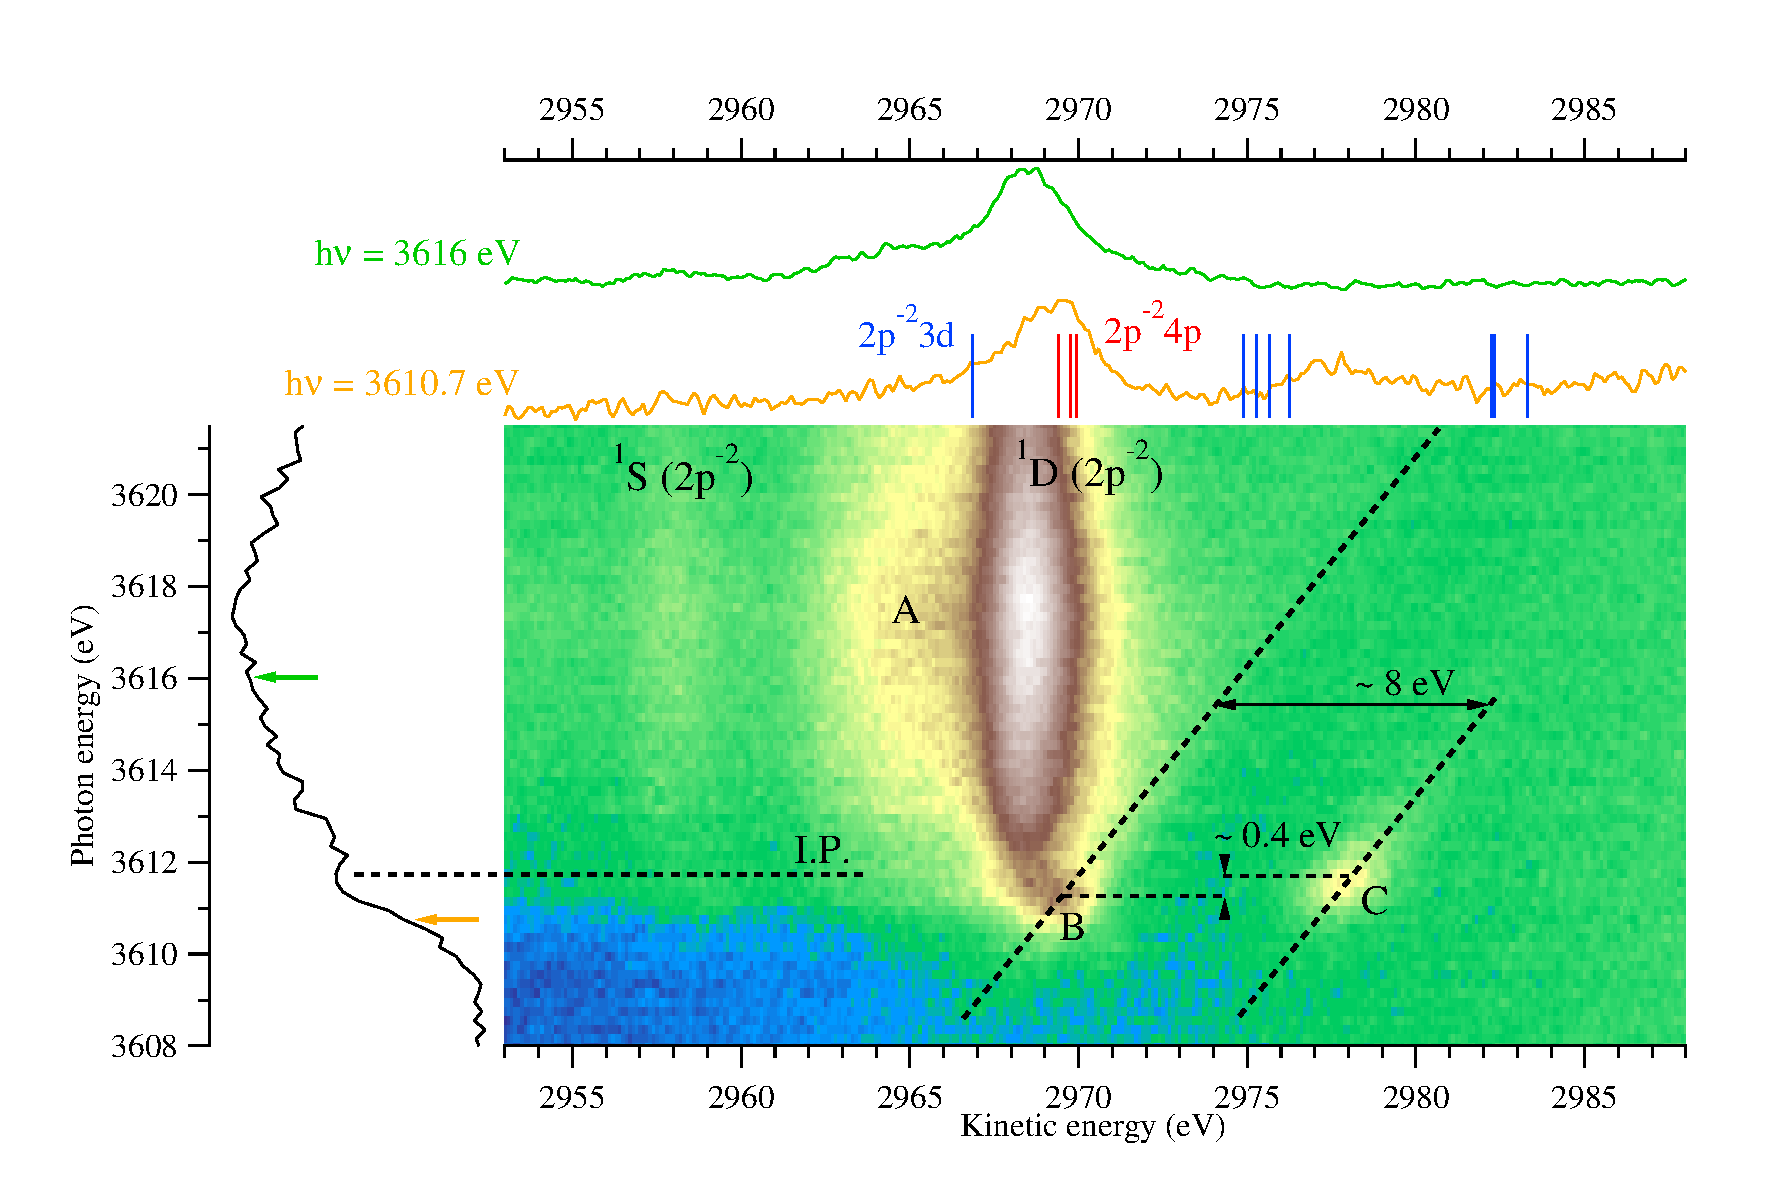
\includegraphics[scale=0.55]{figures/k_2dmap.pdf}
\caption{(a) 2D map showing the kinetic energy of the electrons emitted in KL$_{2,3}$L$_{2,3}$ Auger decay vs the photon energy in the vicinity of the K-edge of aqueous K$^{+}$. The features A, B and C are discussed in the text.
(b) Experimental partial electron yield spectrum of K$^{+}$ obtained after integrating over the kinetic energies of the Auger electrons.
(c) Auger spectra at photon energies 3610.7\,eV and 3616\,eV. The vertical bars in the resonant Auger spectrum measured at 3610.7\,eV indicate the energy positions of the calculated doublet 2p$^{-2}$ 3d (blue) and 2p$^{-2}$4p (red) states of K$^{+}$(H$_2$O)$_6$.}
\label{fg:2dmap_k}
\end{figure}


The KL$_{2,3}$L$_{2,3}$ normal Auger lines may be shifted to higher kinetic energies and also disperse with photon energy close to threshold due to energy exchange between the photoelectron and Auger electron called post-collision interaction (PCI) \citep{russek86:911,guillemin15:012503}. In our spectra, the PCI effect is manifested as an asymmetric tail of the main peaks at photon energies 3616\,eV in the case of \ki, and 2830\,eV in the case of \cli, and as a shift of $\sim$1\,eV of the maxima towards lower kinetic energies as compared to the spectra reported in \citep{ceolin17:263003}. An explanation of the shift is given in the SI.


Finally, the normal Auger $^1$D main line of K$^{+}$ differs from that of Cl$^{-}$ by the presence of a large shoulder on the low kinetic energy side at about 2965\,eV kinetic energy, feature A (Fig.\ \ref{fg:2dmap_k}). This shoulder is attributed to electron transfer from the solvent water molecules to the unoccupied 3d orbitals of K$^{+}$ \citep{ceolin17:263003}. In the case of \cli, there is no experimental evidence of such intense electron transfer processes.


\begin{figure}[h!]
\centering
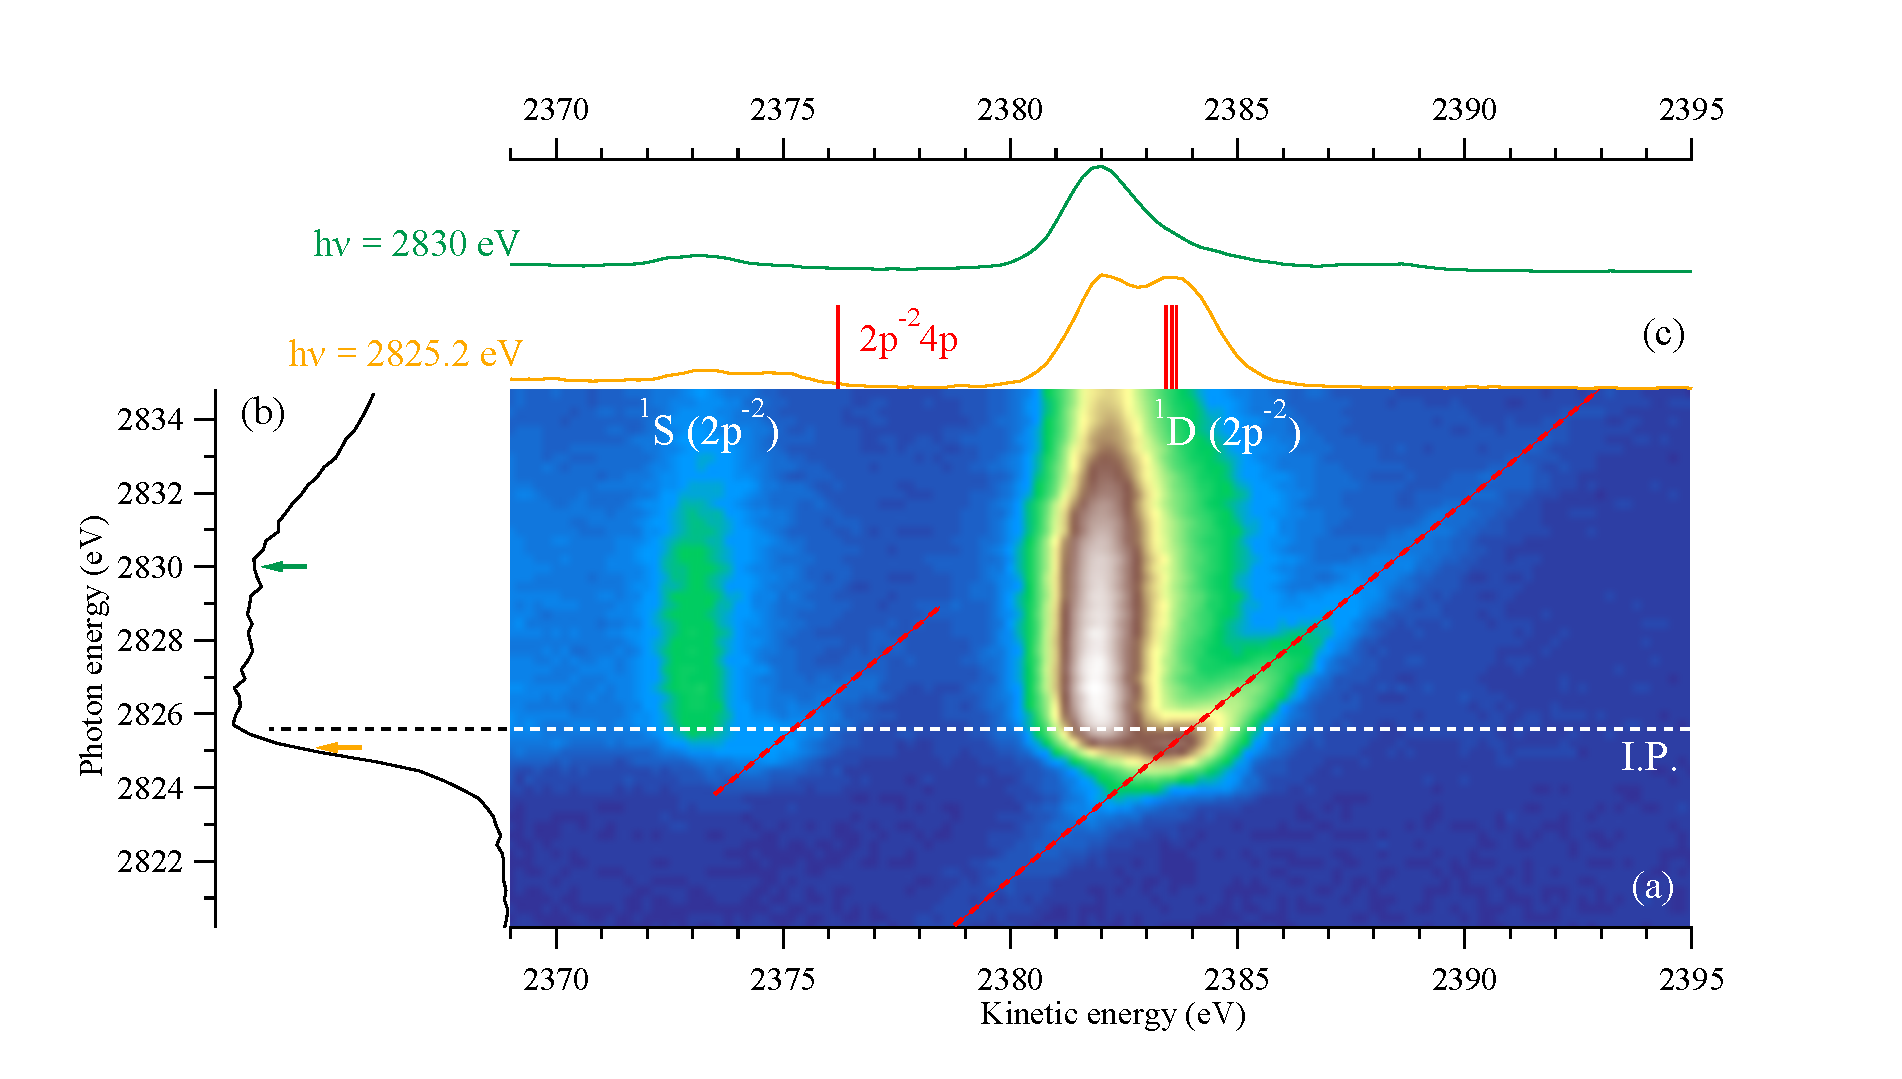
\includegraphics[scale=0.55]{figures/cl_2dmap.pdf}
\caption{(a) 2D map showing the kinetic energy of the electrons emitted in KL$_{2,3}$L$_{2,3}$ Auger decay vs the photon energy in the vicinity of the K-edge of aqueous Cl$^{-}$. 
(b) Experimental partial electron yield spectrum of Cl$^{-}$ obtained after integrating over the kinetic energies of the Auger electrons. 
(c) Auger spectra at photon energies 2825.2\,eV and 2830.0\,eV. The vertical bars in the resonant Auger spectrum at 2825.2\,eV indicate the energy positions of the calculated doublet 2p$^{-2}$4p states of Cl$^{-}$(H$_2$O)$_6$.}
\label{fg:2dmap_cl}
\end{figure}


The KL$_{2,3}$L$_{2,3}$ Auger decay following resonant K-shell excitation of solvated \ki~and \cli~is schematically presented on Fig.\ \ref{fg:auger}. The pre-edge regions of the XAS spectra of \ki~and \cli~do not exhibit any high intensity peaks owing to the lifetime broadening and energetic proximity of the core excited states to the ionization threshold (Figs.\ \ref{fg:2dmap_k} and \ref{fg:2dmap_cl}). Consequently, solely from these spectra, one cannot conclude whether there are core excited states in the pre-edge structure. Instead these states have to be identified by their resonant Auger features, which differ from the normal Auger features. Thus, for \cli, the lowest core excited state is located at 2825.2\,eV, which is in good agreement with the position of the Cl$^{-}$ 1s$^{-1}$4p excitation determined from Cl K-edge XAS experiments \citep{sugiura82:681,shadle95:2259}. In the case of \ki, there are two dispersive features with maxima at photon energies of 3611.2\,eV (B) and 3611.6\,eV (C). The positions of these two core excited states are close to the energy of the 1s$^{-1}$4p excitation in bare \ki~at 3610.7\,eV \citep{hertlein06:062715}.


The resonant Auger features produced in the decay of these core excited states are quite different for \cli~and \ki. In the 2D map of \cli~shown in Fig.\ \ref{fg:2dmap_cl} there are two dispersive features indicated with diagonal dashed lines. The maxima of these features are at 2825.2\,eV photon energy and 2374.6 and 2383.4\,eV kinetic energy, respectively. In the case of \ki, the dispersive line related to the $^1$S main line cannot be clearly identified due to the presence of strong background. Instead two dispersive features related to the $^1$D main line are observed denoted as B and C on Fig.\ \ref{fg:2dmap_k}. Feature B exhibits a maximum at h$\nu = 3611.2$\,eV and 2969.2\,eV kinetic energy. The additional feature C appears at h$\nu = 3611.6$\,eV and 2978.1\,eV kinetic energy, thus it is separated by approximately 400\,meV in photon energy and 8.3\,eV in kinetic energy from the maximum of feature B. 

\begin{figure}[h!]
\centering
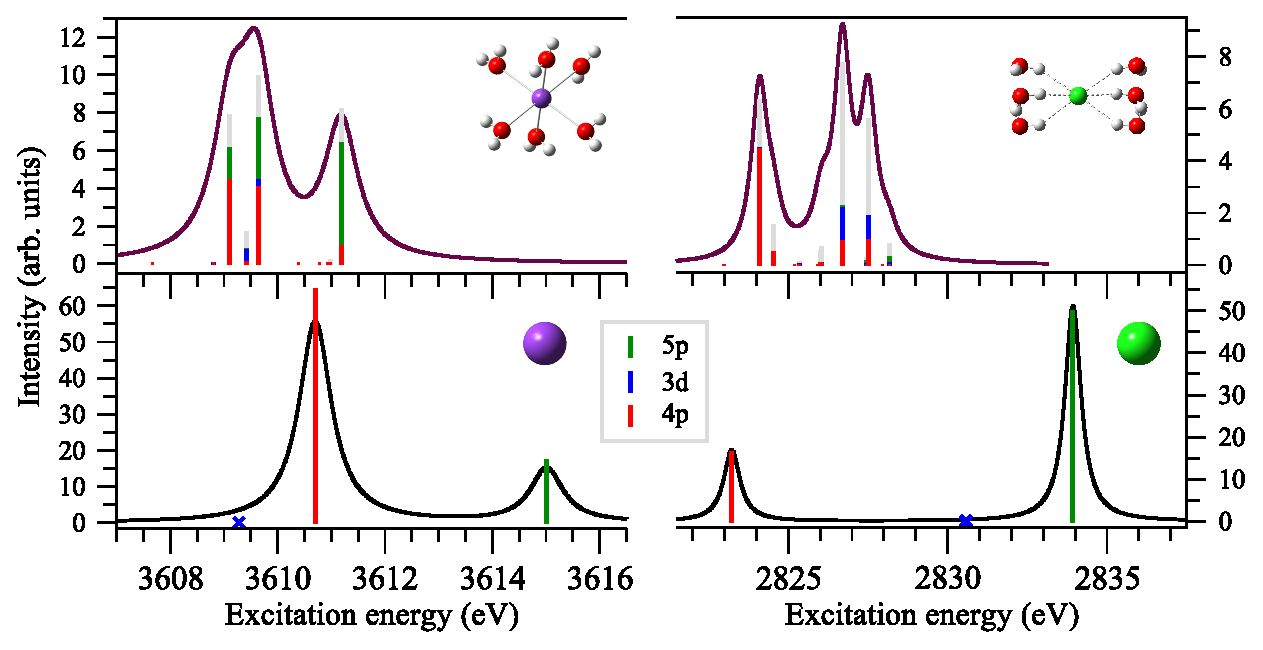
\includegraphics[scale=0.75]{figures/xas_spectra.eps}
\caption{XAS spectra of the lowest K-shell resonant transitions in the bare K$^{+}$ (c) and Cl$^{-}$ (d) ions and their 6-coordinated clusters ((a) and (b)). For comparison with the experiment, the theoretical stick spectra are convolved with a Lorentzian of FWHM  0.74\,eV and 0.62\,eV in the case of \ki~and \cli \citep{Krause79:329} (dashed line)and a Voigt profile (solid line). The stick spectrum corresponds to the projections of the singly-occupied natural orbitals (SONOs) corresponding to the core excited states of the 6-coordinated clusters on the basis of SONOs corresponding to the 1s$^{-1}$3d, 1s$^{-1}$4p, and 1s$^{-1}$5p states of the bare ions. The remaining contributions from higher-lying atomic core excitations or from excitations to the solvent molecules are depicted as grey sticks. The theoretical XAS spectra of both \ki~and \cli~were shifted to higher photon energies such that the energies of the lowest core excited states correspond to the experimentally determined ones. The experimental ionization thresholds are depicted as grey boxes.}
\label{fg:xas_kcl}
\end{figure}


In order to rationalize the pre-edge region of the experimental XAS spectra and the differences in the AES spectra of \ki$_{\text{aq}}$ and \cli$_{\text{aq}}$, we computed the lowest core excited states of the bare \ki~and \cli~ions and their hexa-coordinated clusters (Fig.\ \ref{fg:xas_kcl}). The lowest bright peak in the XAS spectra of the bare ions corresponds to the dipole allowed 1s$^{-1}$4p state followed by the second bright state, 1s$^{-1}$5p, which is located 4.3\,eV and 10.8\,eV higher in \ki~and \cli, respectively. We also show the dipole forbidden 1s$^{-1}$3d states of the bare ions as blue crosses. It is noteworthy that the positions of the 1s$^{-1}$4p and 1s$^{-1}$3d states are inverted in \ki~and \cli, and moreover, the splitting between these states is about two times smaller in \ki, which as explained later is crucial for understanding the Auger spectra of the two ions. Upon addition of water molecules, the degeneracy of the states is lifted, and moreover, they interact with other states of the ion or the neighboring water molecules (Fig.\ \ref{fg:xas_kcl}(a),(b)). Thus, dipole forbidden states acquire intensity in the cluster. A similar effect was observed in the XAS spectra of microsolvated clusters of Na$^{+}$ and Mg$^{2+}$ \citep{miteva16:16671}. Details on the calculations of the XAS spectra are given in the SI.


Further by comparison of the experimental and theoretical XAS spectra, we assume that only the lowest peak in the theoretical XAS spectra is populated in the experiment. In the 6-coordinated \ki~cluster the lowest peak in the spectrum contains three states. The lowest and highest lying states are split by approximately 0.5\,eV and they have mixed 4p and 5p character. The low intensity state lying between these two states has a predominantly 1s$^{-1}$3d character. Since the dispersive feature B appears at low excitation energies, we assume that it is produced in the resonant Auger decay of the lowest core excited states of \ki~of predominantly 1s$^{-1}$4p character. Moreover, we can attribute the feature C to the resonant Auger decay of the low intensity dipole forbidden 1s$^{-1}$3d state. Thus, we explain both the energy splitting of $\sim$400\,meV photon energy of B and C, and the fact that island C has lower intensity than B (Fig.\ \ref{fg:2dmap_k}). In the hexa-coordinated cluster of \cli, the solvent molecules have little influence on the position and character of the first state -- it has mainly \cli~1s$^{-1}$4p character with some admixture of states of the nearest water molecules. We therefore attribute the two dispersive features associated with the $^1$S and $^1$D main lines on the 2D map of \cli~to the resonant Auger decay of this core excited state involving mostly the 4p orbitals of chloride.


To fully characterize the dispersive features on the experimental 2D maps, we also computed the lowest K$^{2+}$[2p$^{-2}$nl](H$_2$O)$_6$ and Cl$^{0}$[2p$^{-2}$nl](H$_2$O)$_6$ doublet states corresponding to the lowest final spectator resonant Auger states. The energy positions of these lines are shown as bars in the upper panels of Figs.\ \ref{fg:2dmap_k} and \ref{fg:2dmap_cl}. In both cases, the lowest 2p$^{-2}$($^1$D)4p states were shifted such that their energies coincide with the maxima of the dispersive features on the high kinetic energy part of the $^1$D main line.

As mentioned above, we attribute the island B on the 2D map of \ki$_{\text{aq}}$ to the decay of the lowest lying core excited state of predominantly 1s$^{-1}$4p character. Supposing that this state undergoes mostly pure spectator resonant Auger decay as in the isoelectronic Ar atom \citep{ceolin15:022502}, then the lowest 2p$^{-2}$4p states are populated resulting in Auger electrons of between 2969.0 and 2970.5\,eV kinetic energy. As can be seen from the Auger spectrum at h$\nu = 3610.7$\,eV (upper panel of Fig.\ \ref{fg:2dmap_k}), the lowest 2p$^{-2}$4p states of \ki(H$_2$O)$_6$ are separated by $\sim$5 and 12-13\,eV from two higher lying groups of 2p$^{-2}$3d states. Thus, the group of 2p$^{-2}$3d states at $\sim$2975\,eV lies closer to the position of island C. Consequently, we attribute this dispersive feature as originating from the resonant Auger decay of the 1s$^{-1}$3d excitation to this group of 2p$^{-2}$3d states. The splitting between the 2p$^{-2}$4p and 2p$^{-2}$3d states in our calculation is smaller than the splitting between the islands B and C. This disagreement can be explained with the fact that we consider a single geometry with a fixed number of water molecules in the first solvation shell, and moreover, we do not theoretically account for the effect of distant solvent shells. Concerning the 2p$^{-2}$3d states at kinetic energies between 2982 and 2983\,eV, we conclude that they are not populated via the Auger process since no additional experimental features are observed.


Another argument in favor of the 2p$^{-2}$3d character of the feature C is the energy difference between the spectral features A and C. Feature A originates from electron transfer processes from water molecules (W) to the doubly core ionized potassium ion and has the configuration K$^{2+}$(2p$^{-2}$3d)W$^{-1}$. The lowest ionization potential of liquid water is about 11.16\,eV \cite{winter04:2625} which fits well with the observed A-C splitting. Thus, the above energetic arguments corroborate the attribution of island C as originating from resonant Auger decay to the K$^{2+}$ 2p$^{-2}$3d final states.


In the computed Cl$^{0}$[2p$^{-2}$nl](H$_2$O)$_6$ spectrum there are two groups of states split by about 7\,eV (upper panel of Fig.\ \ref{fg:2dmap_cl}). The lower kinetic energy group corresponds to the 2p$^{-2}$($^1$S)4p final states, whereas the higher kinetic energy group corresponds to the 2p$^{-2}$($^1$D)4p final states. The splitting between these two groups is in good agreement with the experimental splitting between the dispersive features on the high kinetic energy sides of the $^1$S and $^1$D main peaks. Consequently, we attribute these dispersive features as resulting from the resonant Auger decay of the 1s$^{-1}$4p core excited state of \cli$_{\text{aq}}$ to the 2p$^{-2}$($^1$S)4p and  2p$^{-2}$($^1$D)4p final states.


In summary, we studied the electronic structure of aqueous solution of KCl at the K-edges of both \ki$_{\text{aq}}$ and \cli$_{\text{aq}}$ using a combination of x-ray absorption and Auger electron spectroscopy in the tender x-ray regime, and {\it ab initio} calculations. The Auger electron spectra of both ions exhibit features of both normal and resonant Auger processes. The latter process proceeds differently for aqueous K$^{+}$ and Cl$^{-}$ due to the population of the dipole forbidden K$^{+}$ 1s$^{-1}$3d state in a solution. The spectator Auger decay of this state produces an additional dispersive feature which is manifested as a separate peak in the Auger electron spectrum. In the case of \cli~only fingerprints of the population and Auger decay of the dipole allowed 1s$^{-1}$4p excitation are observed. These results are an important first step in the study of the chains of relaxation steps triggered by x-ray photoabsorption in liquids. The Auger processes considered here are inevitably followed by multiple intra- and interatomic electronic decays, such as interatomic Coulombic decay (ICD) and electron-transfer mediated decay (ETMD) \citep{unger17:708,Stumpf16:237}. As a result of the latter processes, genotoxic free radicals and slow electrons are formed in the vicinity of the metal center. The magnitude of the damage inflicted upon the environment and the energies of the emitted electrons depend on the initial Auger step, and can therefore be controlled by tuning the energy of the radiation. Consequently, the results of this work can have implications in understanding radiation chemistry and radiation damage in biologically relevant systems in which metallic centers are ubiquitous.